\chapter{基于深度学习的用户语义理解}

\section{语义理解任务描述与解决流程}
\subsection{问题描述}
跨界服务平台内服务的智能调用实现过程中,语义理解是关键。系统接收的是用户输入的一句有目的性的话,系统在语义理解的过程中,
首先要识别用户的意图,根据
用户意图匹配相应的服务以及匹配该服务要执行的操作,这两者均可被视为文本分类问题,可以用深度学习的分类算法解决,
再本文被称作服务分类和接口分类任务;找到匹配的服务以后,在服务执行前需要
必要的执行参数,可以从用户输入的语句中提取,这将被看作语义槽填充问题,可以用序列标注算法解决,
将词语序列x=[$x_{1}$,$x_{2}$,\dots,$x_{T}$]映射到相应的插槽标签序列y=[$y_{1}$,$y_{2}$,\dots,$y_{T}$],再本文被称作参数提取任务。

以调用火车票信息查询服务为例,来解释跨界服务平台内服务分类,接口分类和参数提取。
用户在进入跨界服务平台后,输入“查询成都前往杭州的火车票”,跨界服务平台内
的语义理解模型识别出该语义对应平台内部的<train服务>,接口类型为<query查询>,语义槽(即服务参数)为<startCity起始地>成都和<endCity目的地>杭州。


\begin{figure}[htbp]
    \centering
    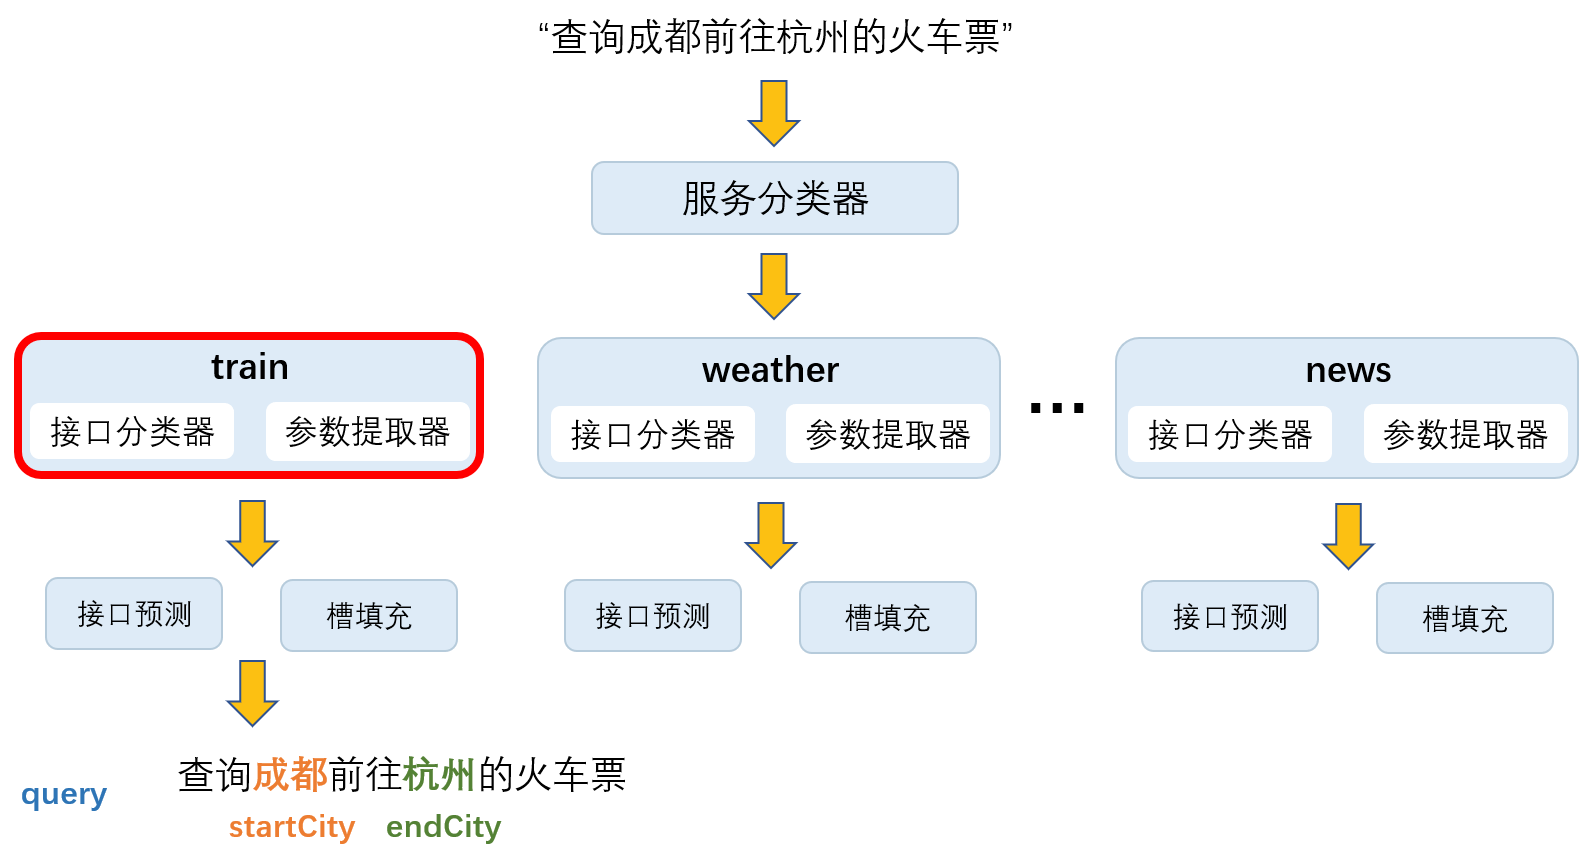
\includegraphics[scale=0.5]{./images/liucheng.png}
    \caption{语义理解算法流程}
    \label{fig:questiondesc}
  \end{figure}

\subsection{算法描述}
基于深度学习的语义理解算法,首先将用户输入的句子利用分词工具转化为词语序列,再用word2vec将词语向量化,
固定句子长度后,得到结构化的表示形式x=[$x_{1}$,$x_{2}$,\dots,$x_{T}$]输入网络中,流程如图\ref{fig:questiondesc}所示。
首先利用服务分类器得到系统内与用户意图相匹配的服务,再通过接口分类器和参数提取器分别做文本分类和语义槽填充处理,最后将三项任务得到
的结果提交至服务执行引擎做服务调用,算法详细描述如表\ref{tab:suanfa1}。

\begin{table}[htb]
  \centering
  \caption{基于深度学习的语义理解算法描述}
  \label{tab:suanfa1}
\begin{tabular}{p{150mm}}
\toprule
\textbf{算法1:}基于深度学习的语义理解\\
\textbf{输入:} $L_0$=\{($S_i$,$y_i^d$,$y_i^i$,$y_i^s$)\},i $\in$ [1,n]\\
\textbf{输出:} $Model_{service}$,$Model_{interface}$,$Model_{slot}$\\
\hline
\textbf{过程描述:}模型在训练时,输入的$S_i$为有用户意图的语句,经过分词和向量化
处理后得到$E_i=(e_1,e_2,\dots,e_T)$,T为词语个数。模型参数初始化、批处理的数量
iterations = M 和每一批的样本数 batchsize、迭代次数 epoch = N 和当前迭代次数 i = 0\\
\textbf{while} i < N or 模型的性能达到终止条件 \textbf{do}\\
\qquad \qquad \textbf{for} j = 1,\dots ,M \textbf{do}\\
\qquad \qquad \qquad \qquad 随机抽取 batchsize 个训练集数据,前向传输在当前网络权值和输入下网络的输出\\
\qquad \qquad \qquad \qquad 反向传输调整模型参数\\
\qquad \qquad \textbf{end for}\\
\qquad \qquad 计算损失 Loss,更新梯度和模型的参数\\
\textbf{end while}\\
用训练好的领域分类模型对测试样本进行预测,加载训练好的相应领域的意图识别模型
和语义槽填充模型,对意图和语义槽进行预测,计算准确率 Accuracy、损失 Loss\\
\bottomrule
\end{tabular}
\end{table}

\section{预处理}
\subsection{序列化}
% 结巴分词,word2vec
% 用户不需要输入完整的句子
神经网络的输入是一个向量序列,但用户输入是一个完整的句子,因此首先需要把句子序列化,之后使用word2vec将词语向量化。
本文采用结巴分词来做序列化的处理,
结巴分词分了三种模式,准确模式试图将句子切成最贴切的句段,适用于文本分析;完全模式会从句子中获取所有可能的单词,速度快但不精确;
基于准确模式的搜索引擎模式试图将长词切成几个短词,从而提高查全率,适用于搜索引擎。
结巴分词的算法依据主要是基于前缀字典结构来实现高效的词图扫描,为所有可能的单词组合构建有向无环图(DAG),
使用动态规划根据单词频率查找最可能的组合。

本文在实际处理中发现文本的预处理特别重要,如果句子中包含了太多无关词(这些词被称作停用词),算法性能会受影响,因此本文
在文本预处理时引用了停用词过滤。比较常见的中文停用词如“的”、“在”以及语气词等,他们的存在对语义理解没有贡献,相反如果分词工具使用他们错误的分词,
会降低模型准确率,因此本文利用网上已有的中文停用词词典在结巴分词工具处理前对用户语句做了停用词过滤。

\subsection{标签向量化}
服务分类和接口分类均属于多类别分类问题,训练样本的标签均采用one-hot编码,本文筛选了跨界服务平台中用户使用较多的八类服务,接口类型为这八类
服务下所有接口的合计,如query,order,play等。对于参数提取任务,像序列标注任务一样,使用BIO标注方式标记参数语义槽,根据类型不同分为
“B-X”、“I-X”和“O”,如图\ref{fig:yuyicao}所示。
\begin{figure}[htbp]
  \centering
  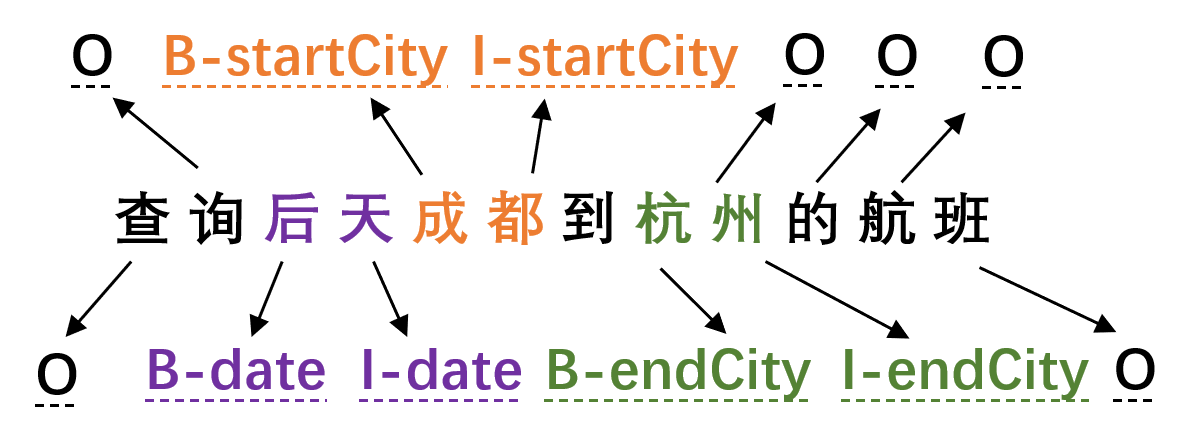
\includegraphics[scale=0.5]{./images/yuyicao.png}
  \caption{参数语义槽标注}
  \label{fig:yuyicao}
\end{figure}


\section{基于attention-CNN-LSTM的服务分类模型}
实现服务智能调用的第一步要根据用户意图匹配相应的服务,这可以被转化为文本分类问题。
LSTM
是一种特殊的RNN,能够学习长期依赖关系,理解关键字出现的顺序,擅长处理文本序列的问题,同时,
它通过增加门机制来过滤信息,解决了长距离依赖的问题。 另一方面,在某种程度上也避免了梯度消失和梯度爆炸的问题。
CNN
多用于图像领域,由于卷积核的存在,能够提取出词与词之间的隐藏的语义信息,捕获局部相关性。
尽管CNN可以在许多任务中很好地表现,但它最大问题之一是卷积核大小的在训练时固定,不具有很好的泛化能力,一方面,无法对更长的序列信息进行建模,
另一方面,超参数卷积核大小的调整也增加了工作量,Max pooling丢失了结构性信息,因此很难在文本中发现复杂的模式。
为了
能让卷积层从单词嵌入向量中提取更高级别的短语表示,我们在模型中引入attention层.这是因为在传统的CNN中,有效地编码长期上下文信息和非连续词之间的相关性并不容易,
它仅考虑在表面字符串上连续的连续n-gram,因此忽略了非连续词之间的某些长距离相关性,而这种相关性在许多语言中都起着重要作用。比如,用户输入“帮我挂
明天上午邵逸夫医院的号”,这里“挂”和“号”显然应该组合在一起成词才能具有完整正确的语义信息。同时,NLP中有关注意力的大多数现有研究都集中在对不同模式之间的相关性进行建模,
例如机器翻译中源语言和目标语言之间的单词对齐以及问答中问题与答案之间的单词相似性。在本文中,我们将attention层放在卷积层之前,
注意力机制用于自动捕获长期上下文信息和非连续词之间的相关性,而无需任何外部语法信息。

综上所述本节将三者结合各取所长, 采用ATT-CNN-LSTM模型\ref{fig:cnn-lstm}用以解决服务分类问题,下面将详细介绍该模型

\begin{figure}[htbp]
    \centering
    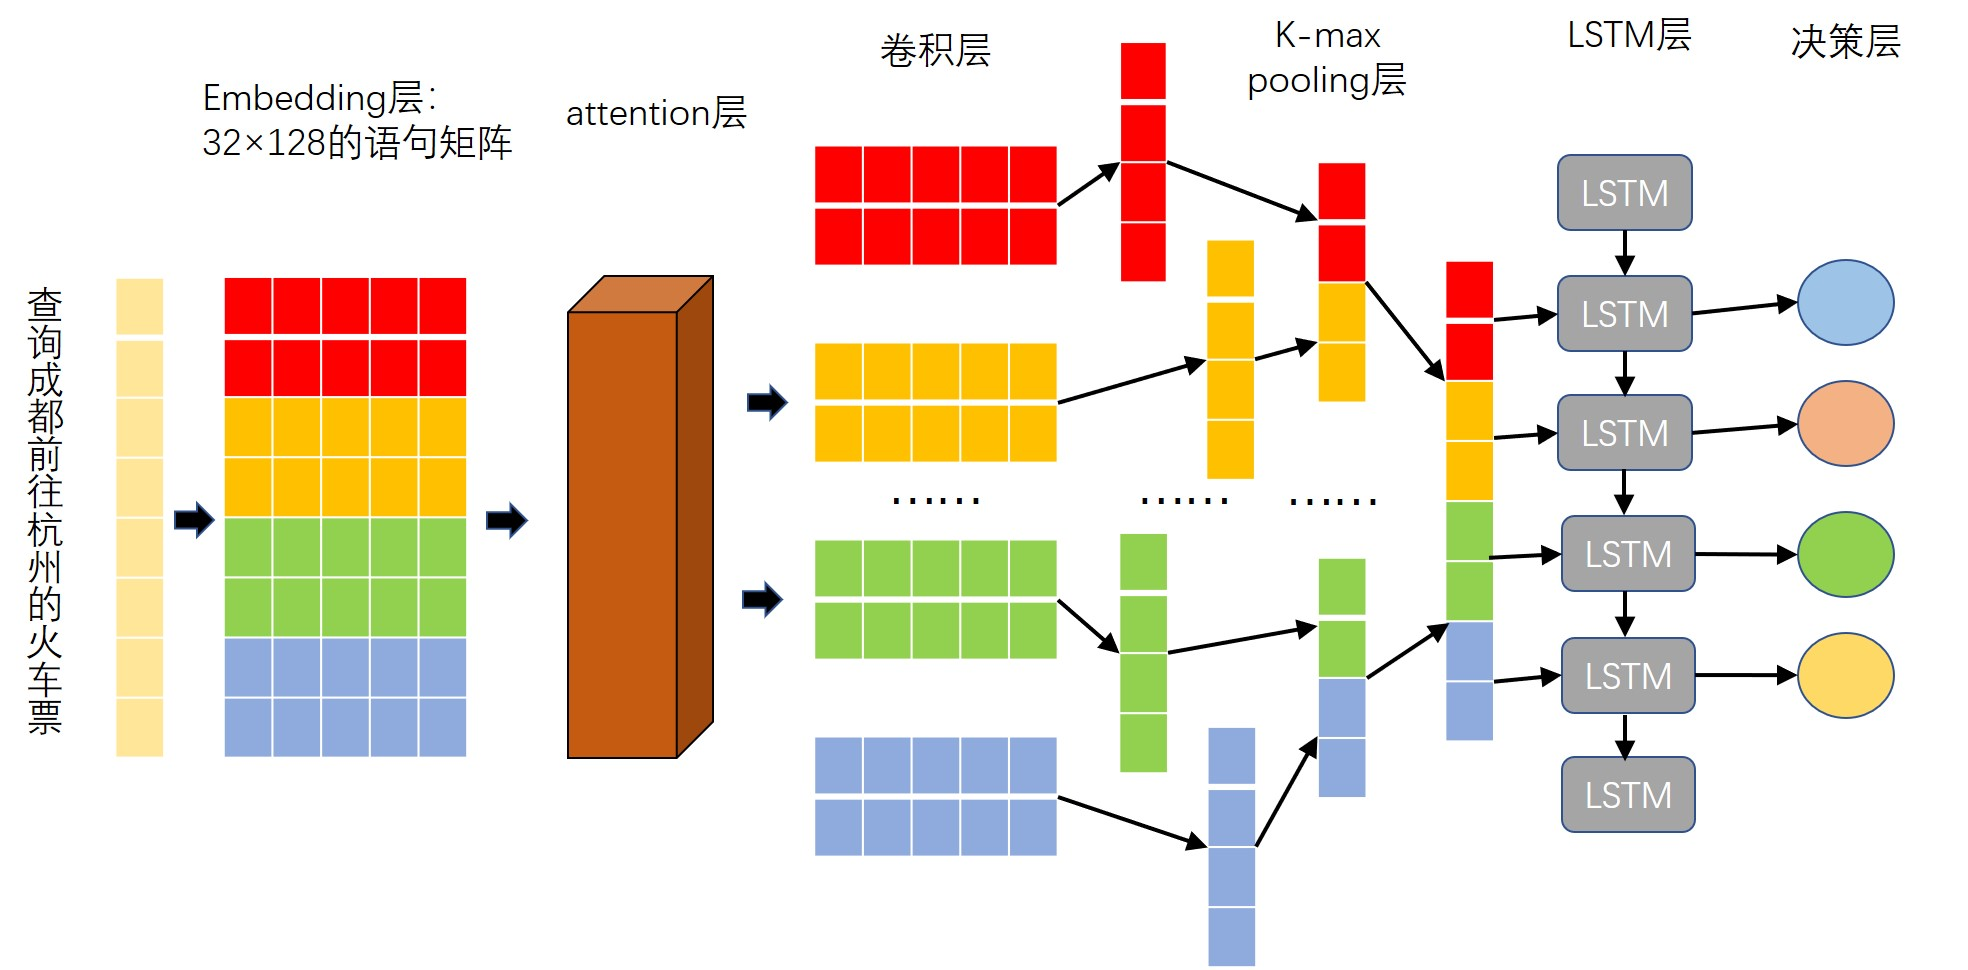
\includegraphics[scale=0.5]{./images/cnn-lstm.jpg}
    \caption{服务分类模型}
    \label{fig:cnn-lstm}
  \end{figure}


  1)输入层与embedding层

  用户输入的语句通过结巴分词工具得到中文词的模型即可完成输入层的任务到达embedding层。之后将文本序列转换为矢量形式的数字表示,word2vec是最常用的方法之一。
  在本实验中,我们选择通过C-BOW模型基于维基百科中文语料库预训练得到的word2vec模型,通过使用预训练词向量模型可以有效地减少人工神经网络的过度拟合。
  由于神经网络的输入长度在本模型中是固定的,加之用户输入的语句长度通常有限,结合数据集中最长句子拆分以后的序列长度考量,我们决定把最大长度设为32.
  同时word2vec模型的输出的词维度为128维,因此每一个需要匹配系统内服务的用户输入的句子就构成了一个32×128的二维矩阵E=[$e_{1}$,$e_{2}$,\dots,$e_{32}$],
  其中$e_{i}$=[$e_{i1}$,$e_{i2}$,\dots,$e_{i128}$]是一个中文词经过word2vec处理的向量表示。

  2)attention层

  如图\ref{fig:att-cnn}所示,是注意力层的主要结构,在输入层和卷积层之间引入了注意层.具体而言,注意力层是为每个词创建上下文向量。,
  上下文向量与词向量串联在一起,作为新的词表示形式将被输入到到卷积层。 凭直觉,一对彼此远离的词往往联系较少,因此,我们将距离衰减添加到注意力机制中。 
  注意机制的思想是在推导$x_{i}$的上下文向量$g_{i}$时将注意力集中在特定的重要单词上,图\ref{fig:att-cnn}中的红色矩形代表$g_{i}$。 
  注意机制是一个附加的多层感知器,它与ATT-CNN-LSTM的所有其他组件共同训练,这种机制确定了在预测服务类别时哪些词应比句子上的其他单词获得更多的关注。
  注意力机制生成的上下文向量$g_{i}$由一下公式得到:
  \begin{equation}
  \mathbf{g}_{i}=\sum_{j \neq i} \alpha_{i, j} \cdot \mathbf{x}_{j}
\end{equation}
其中,$\alpha_{i, j}$是注意力权值,其计算方式如下:
\begin{equation}
\alpha_{i, j}=\frac{\exp \left(\operatorname{score}\left(\mathbf{x}_{i}, \mathbf{x}_{j}\right)\right)}{\sum_{j^{\prime}} \exp \left(\operatorname{score}\left(\mathbf{x}_{i}, \mathbf{x}_{j^{\prime}}\right)\right)}
\end{equation}
\begin{equation}
\text { score }\left(\mathbf{x}_{i}, \mathbf{x}_{j}\right)=v_{a}^{\top} \tanh \left(W_{a}\left[\mathbf{x}_{i} \oplus \mathbf{x}_{j}\right]\right)
\end{equation}
词与词之间的score值由感知器计算得到,我们以此来度量词与词之间的相关性,得分越高表示相关性越强。
经过这一层的处理,用户输入的句子被转换为32×256的二维矩阵A=[$a_{1}$,$a_{2}$,\dots,$a_{32}$],
其中$a_{i}$=[$a_{i1}$,$a_{i2}$,\dots,$a_{i256}$]是一个中文词经过attention处理的向量表示。

\begin{figure}[htbp]
  \centering
  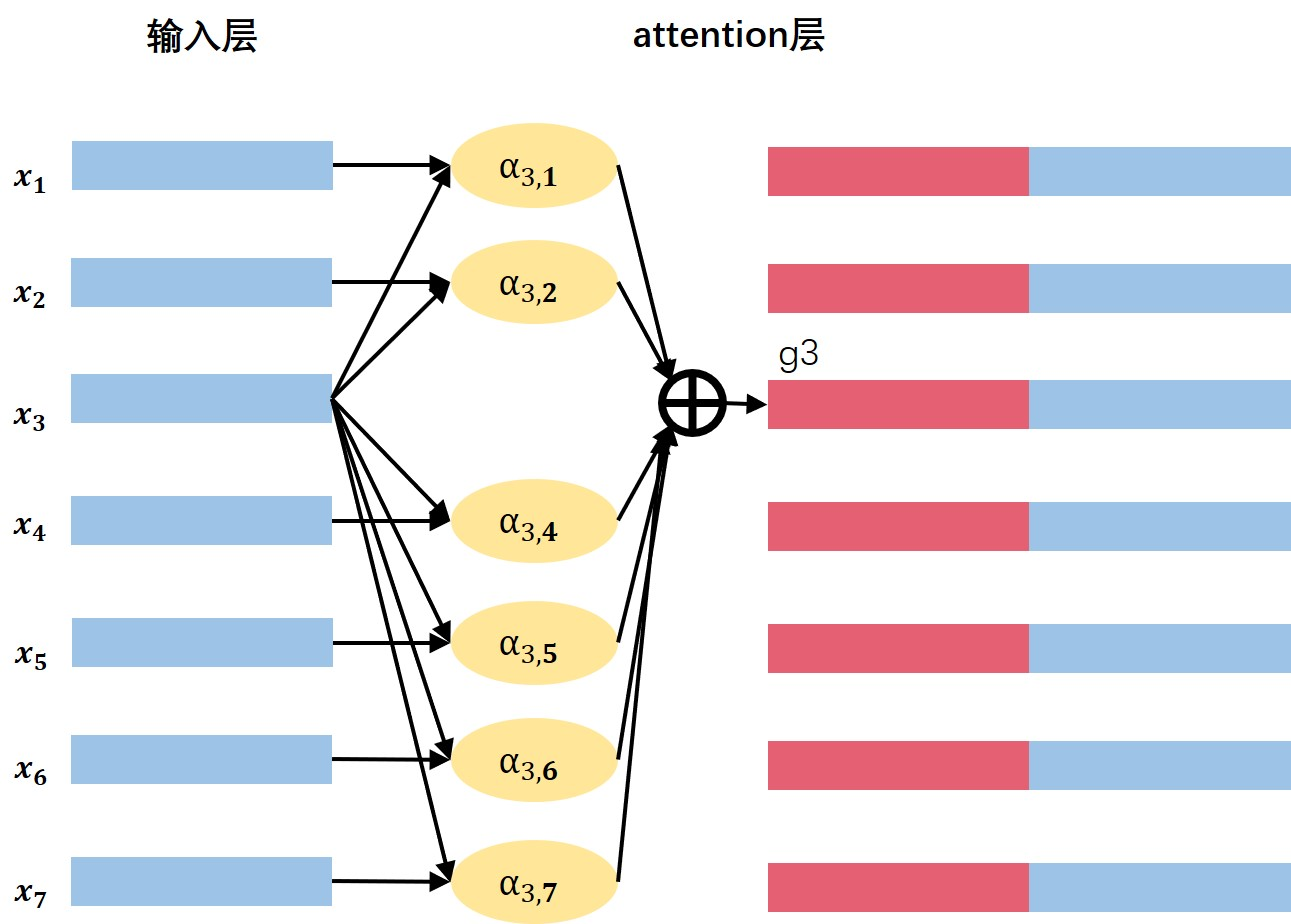
\includegraphics[scale=0.4]{./images/attcnn.jpg}
  \caption{服务分类模型中attention层}
  \label{fig:att-cnn}
\end{figure}
  3)卷积层

  由于卷积核的存在,卷积层能够提取出词与词之间的隐藏的语义信息,捕获局部相关性。这里我们仅设置了单层的卷积层,用于捕获序列局部信息并对输入数据的降维。
  设置不同初始化权重的多个卷积核用于提高模型的学习能力,本模型共设置了64个卷积核,卷积核在文本矩阵上移动以提取特征。在文本处理领域CNN的卷积操作常被设置
  为一维卷积,这是因为直观上来看沿着词向量所在的维度不具有拆分性,因此卷积核总是沿着词与词之间的维度扫面提取特征,对m×n的矩阵以高为h的卷积核做一维卷积
  会得到一个高为m-h+1,宽为1的长条状矩阵。基于此,本文卷积核宽度与attention输出层
  一致为256,高度设置了[2,3]三种选择以期获得不同维度的语义信息,所以本层的输出结果大小随卷积核的尺寸不同会不一致,即会得到64个大小不一的矩阵称为feature maps.
  卷积操作的计算公式如下:
  \begin{equation}
    c=ReLU(W_{c}A+b_{c})
    \end{equation}
    这里选用ReLU作为非线性激活函数,可以改善网络的学习动态并显着减少深度网络中收敛所需的迭代次数,c为一个卷积核做一次卷积运算所得值。

  4)pooling层

    如上层所述,卷积层的输出结果大小随卷积核的尺寸不同会不一致,因此pooling层有统一维度的作用。
    同时可以降维降低计算复杂度,保留核心特征,减少模型参数防止过拟合提高模型泛化能力。
    由于卷积核卷积操作得到的结果是长条状,因此本文采用k-max pooling池化方法,k是超参数,设置为4。经过池化层处理后,得到4×64的特征矩阵作为lstm层的输入。
  从64维的角度来看,每一维是一种高层语义特征的提取。

    5)lstm层

  直观上,文本分类是顺序信息处理的过程。但是,从卷积神经网络以并行方式获得的特征序列不包含序列信息,LSTM专为顺序建模而设计,
  可以进一步从CNN获得的特征序列中提取上下文信息,lstm内部核心计算过程如下:
  \begin{equation}
  f_{t}=σ(W_{f}\cdot[h_{t-1},x_t]+b_{f})
  \end{equation}
  \begin{equation}
    C_{t}=f_{t} * C_{t-1}+i_{t} * \tilde{C}_{t}
    \end{equation} 
    \begin{equation}
      o_{t}=\sigma\left(W_{o}\left[h_{t-1}, x_{t}\right]+b_{o}\right)
    \end{equation} 
    \begin{equation}
      h_{t}=o_{t} * \tanh \left(C_{t}\right)
    \end{equation}
    其中,$x_t$为从池化层输入的变量,其他字符代表的是lstm内部计算的中间过程变量不再赘述,得到的结果$x_t$被输入到下一层
  6)优化层与决策层


可以认为,矩阵分别经过卷积层和LSTM层后,可以获得高度提取的语义信息。



\section{基于Transformable-CNN-LSTM的接口分类模型}
接口分类和服务分类本质上一样都可以视为文本分类问题,我们在处理接口分类问题时没有生搬硬套服务分类模型,而是希望改进以提升性能,因此做了不同的尝试。
CNN在许多自然语言处理任务中都很有效,常规的CNN不可避免地面临适应特征变换的挑战,这是由于CNN具有许多几何上固定的结构,
例如卷积层将卷积层形状限制为n-gram,而pooling层会使用solid chunks提取高层语义特征。这些固定的结构为语言表示带来了两个主要限制:所有卷积核和块都是连续的且形状固定的,
这使CNN难以处理某些复杂的情况,例如非连续或过大的特征,换句话说,它处理不了不符合卷积核形状的特征,传统的CNN无法主动进行调整以适应特征的转换。
他们倾向于记住大型数据集中特征各种形式的变体,但不了解特征的转换。举个例子,
给定短语“不那么好”,传统的卷积网络很难直接捕获非连续模式“不...好”,也很难从许多转换形式中识别出这种模式,例如“不太好”,此即为“不好”这个特征的转化表达。

本节采用了端到端的文本分类模块,分别修改了传统卷积层和传统池化层,称作可转换卷积和可转换池,两个模块都可以增强CNN对转换特征的建模能力。
可变换卷积将一维偏差信息添加到卷积核的采样位置,这不仅可以帮助捕获复杂特征,而且可以抵消特征变换。
神经网络可以自动学习偏差,而无需额外的监督或人工经验,可转换池与可转换卷积有着相似的思路。
在传统池化层的基础上,它将一维偏差添加到块的采样位置,以增加特征选择的适应性。
在本节中,我们重点介绍两个可转换模块,这些模块具有可学习的形状以适应特征的变化。 
通常,卷积和池化中的卷积核和块的形状从一开始就是固定的,因为时超参数。 但是可转换模块将学习到的位置偏差信息添加到卷积核或块上,从而使其形状灵活,适应性增强。 
位置偏差信息由动态部分和静态部分组成,在预测阶段,动态偏差与当前输入有关,其值可从当前特征中主动获取以捕获特征转换信息。 
相反,静态偏差值像其他权值一样通过反向传播进行更新,并在预测阶段保持不变,这描述了特征信息的全局基本分布。
同时lstm能够学习长期依赖关系,理解关键字出现的顺序,擅长处理文本序列的问题.我们把lstm拼接在可转换卷积层之后对语义信息做进一步的处理,
这个接口分类的模型如图\ref{fig:tran-cnn-lstm},下面将详细介绍该模型:

\begin{figure}[htbp]
  \centering
  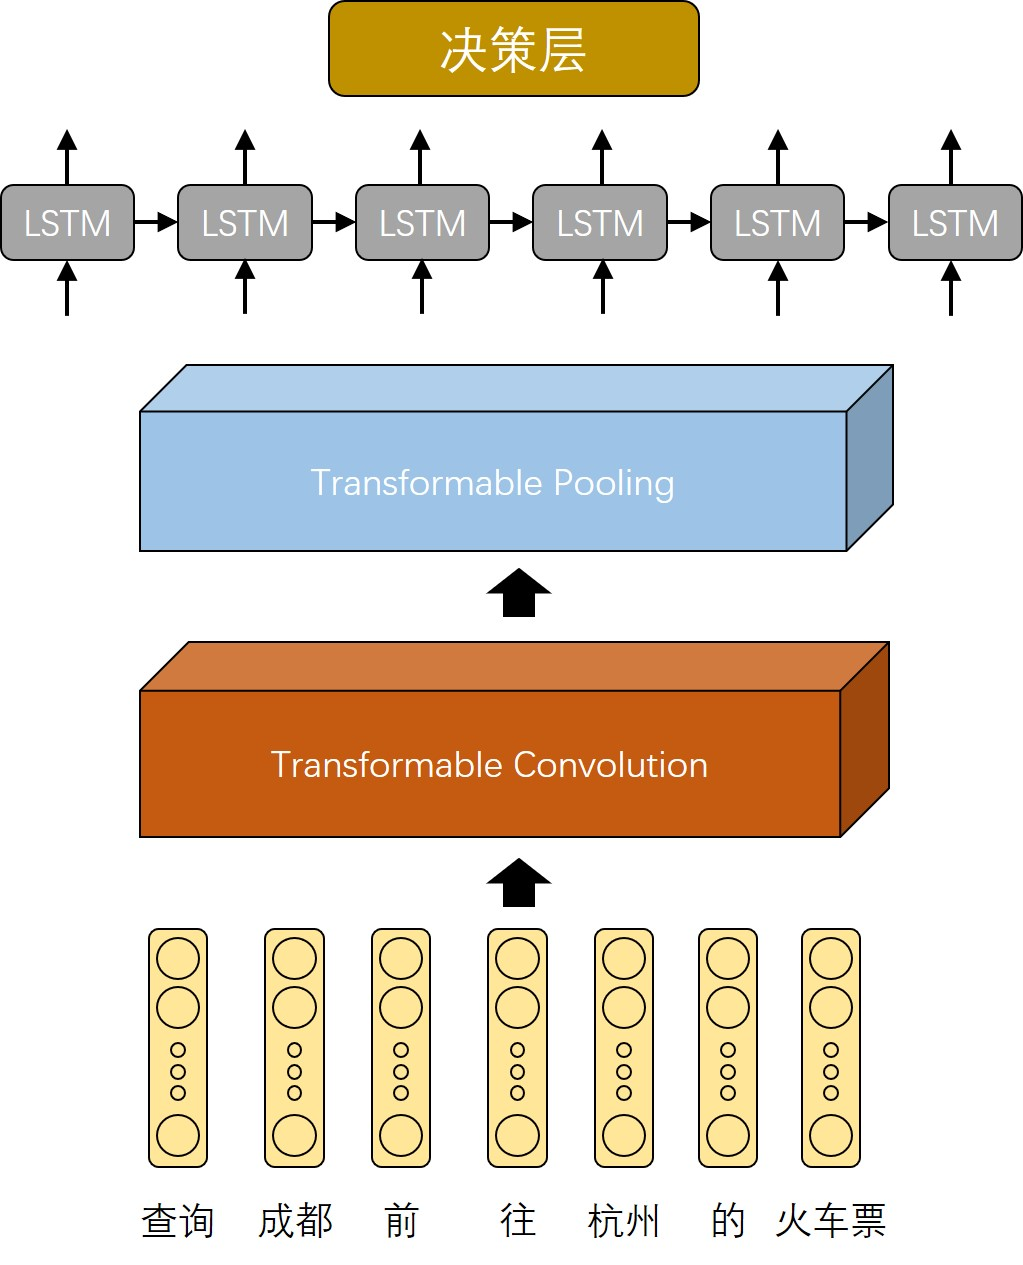
\includegraphics[scale=0.4]{./images/tran-cnn-lstm.jpg}
  \caption{接口分类模型}
  \label{fig:tran-cnn-lstm}
\end{figure}

1)输入层与embedding层

该层与服务分类模型做相同处理,不再赘述。需要注意的是与上一个模型有一处不同,我们选择输出维度为256维的词向量模型,序列长度仍为32,
因此每一个需要匹配系统内服务的用户输入的句子就构成了一个32×256的二维矩阵E=[$e_{1}$,$e_{2}$,\dots,$e_{32}$],
其中$e_{i}$=[$e_{i1}$,$e_{i2}$,\dots,$e_{i256}$]是一个中文词经过word2vec处理的向量表示。


2)可转换卷积层

对于传统CNN的卷积核大小是固定,卷积核在对输入图像扫描过程中每一次卷积操作的范围是固定的,如图\ref{fig:tansconv}的左图所示,一次普通的卷积运算可以用以下公式表示:
\begin{equation}
  y=\mathbf{w}\mathbf{x}
  \end{equation}
  将上式展开计算卷积核中每一个元素,公式被转换为:
  \begin{equation}
    \mathbf{y}\left(p_{0}\right)=\sum_{p_{i} \in \mathbf{C}} \mathbf{w}\left(p_{i}\right) \cdot \mathbf{x}\left(p_{0}+p_{i}\right)
    \end{equation}
其中,C为本次卷积核采样的全集,$p_{0}$是卷积运算后本次卷积在结果特征图中的位置,$p_{i}$枚举了本次卷积核采样的全集中的所有位置,并且
表示与$p_{0}$的距离。
在可转换卷积(transformable convolution)中,一次卷积运算的采样全集C被分为两部分,分别用$\mathbf{D}_{c} \subset \mathbf{C}$和
$\mathbf{S}_{c} \subset \mathbf{C}S$来表示,$\mathbf{D}_{c}$是与当前输入特征相关的动态位置偏移信息,$\mathbf{S}_{c}$是训练时得到的
由全局觉得的静态位置偏移信息。然后这两部分在计算时分别被加上不同的位置偏移值$\Delta p_{i}^{\mathbf{D}_{c}}$和$\Delta p_{i}^{\mathbf{S}_{c}}$,
这样卷积的计算公式就变成了:
\begin{equation}
  \mathbf{y}\left(p_{0}\right)= \sum_{p_{i} \in \mathbf{D}_{c}} \mathbf{w}\left(p_{i}\right) \cdot \mathbf{x}\left(p_{0}+p_{i}+\Delta p_{i}^{\mathbf{D}_{c}}\right) +\sum_{p_{i} \in \mathbf{S}_{c}} \mathbf{w}\left(p_{i}\right) \cdot \mathbf{x}\left(p_{0}+p_{i}+\Delta p_{i}^{\mathbf{S}_{c}}\right)
\end{equation}
现在,$\mathbf{D}_{c}$和$\mathbf{S}_{c}$的引入,卷积核的采样位置能够做到动态的变化,实现了重新分布,而不是像以前一样是固定的矩形。
考虑到$\Delta p_{i}^{\mathbf{D}_{c}}$和$\Delta p_{i}^{\mathbf{S}_{c}}$往往是小数,因此$\mathbf{x}()$的计算采用线性插值的方法:
\begin{equation}
\mathbf{x}(p)=\sum_{q} K(p, q) \cdot \mathbf{x}(q)
\end{equation}
这里p代表$p_{0}+p_{i}+\Delta p_{i}^{\mathbf{D}_{c}}$或者$p_{0}+p_{i}+\Delta p_{i}^{\mathbf{S}_{c}}$,q枚举了输入矩阵的所有位置,
K是线性插值运算的核:
\begin{equation}
K(p, q)=\max (0,1-|p-q|)
\end{equation}
图\ref{fig:tansconv}显示了可变换卷积的机制,顶部的动态位置偏差$\Delta p_{i}^{\mathbf{D}_{c}}$是通过一个普通的卷积层从当前输入序列中计算得到的,
其值被添加到$\mathbf{D}_{c}$中的采样位置。 由于它们是从输入计算生成的,因此它们的值会根据当前特征动态变化,以适应当前的转换模式。 
底部的静态偏差$\Delta p_{i}^{\mathbf{S}_{c}}$是变量,在训练阶段通过反向传播进行更新,并在预测时保持不变,因此,静态偏差描述了特征的全局分布。
共设置了128个卷积核,宽度与词向量长度一致,高度分为[2,3,4]不等,选用ReLU作为非线性激活函数,本层结束将得到128个大小不一的长条状feature maps.


\begin{figure}[htbp]
  \centering
  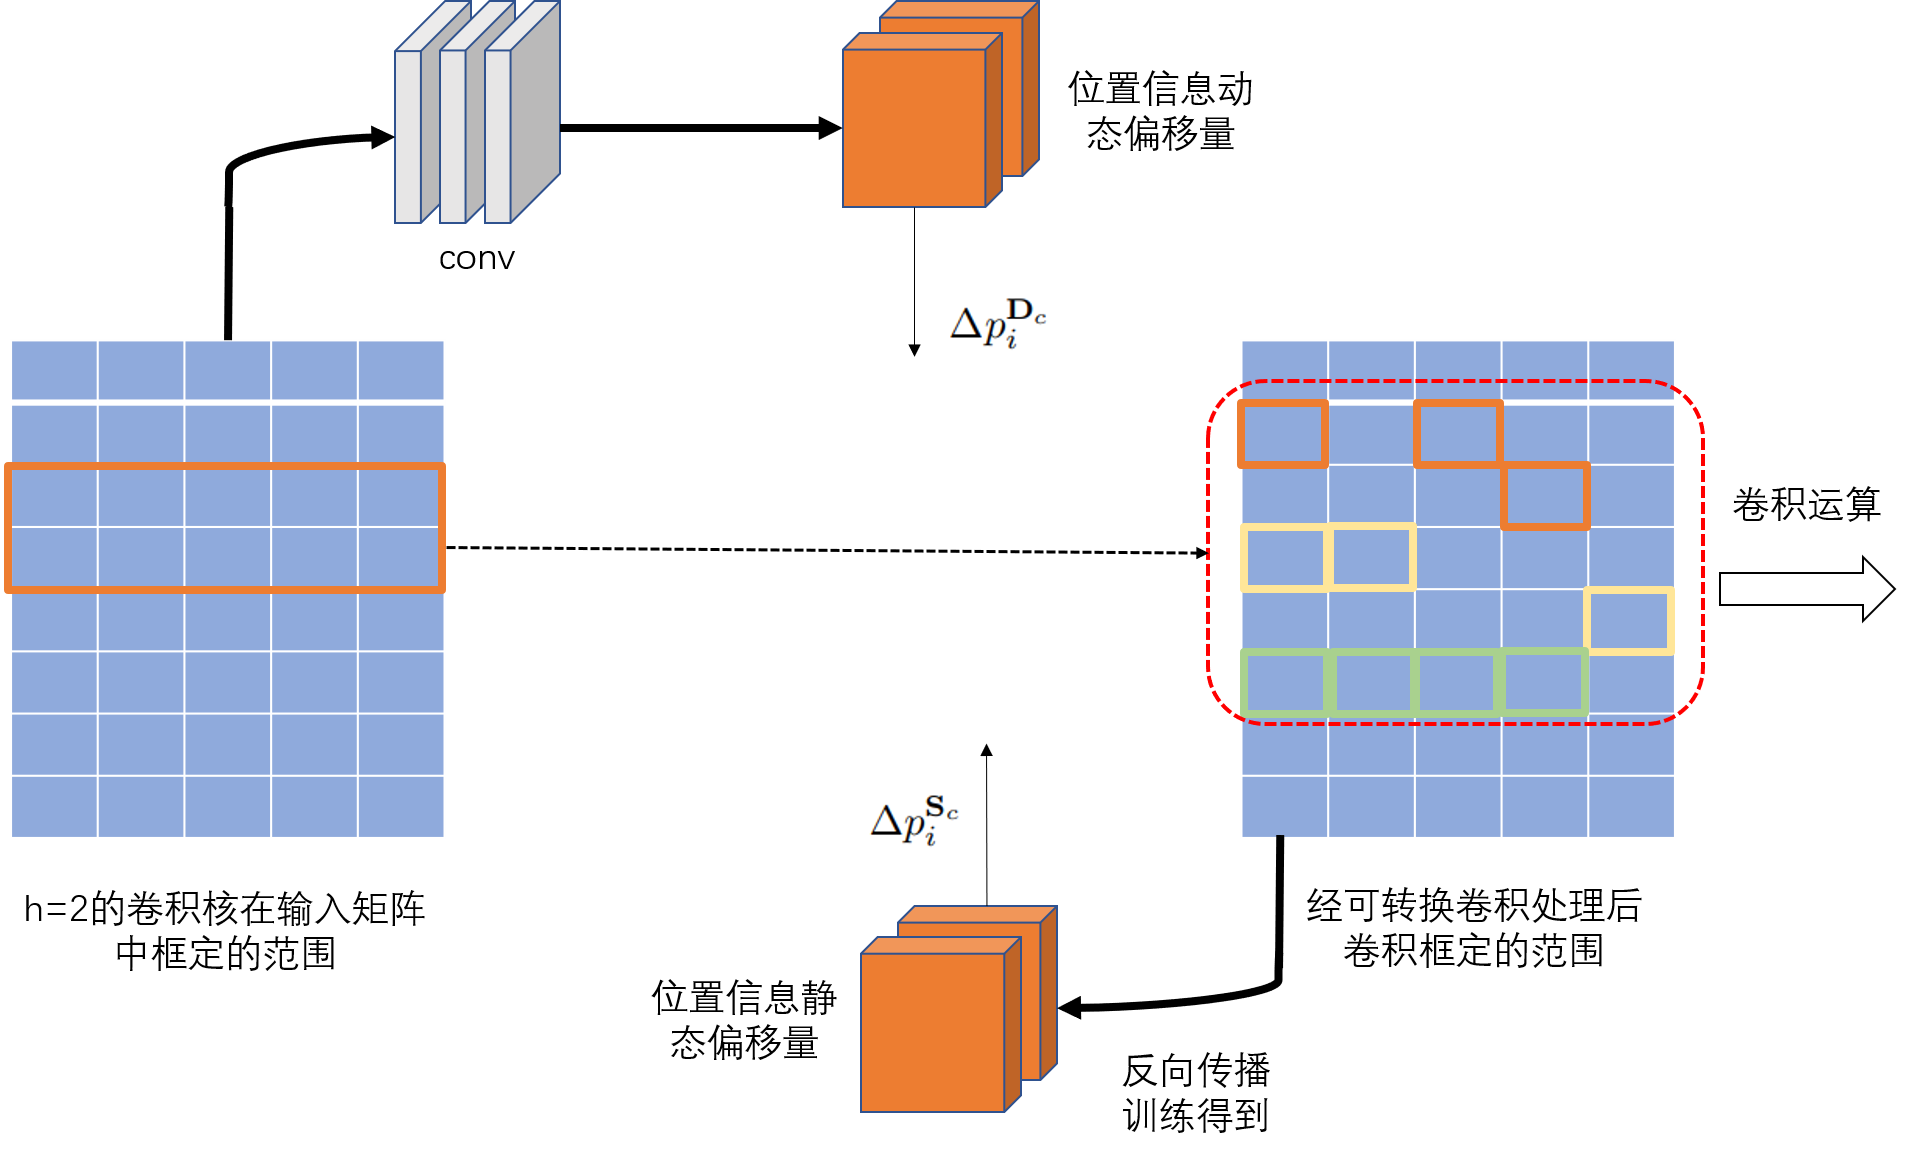
\includegraphics[scale=0.4]{./images/tansconv.jpg}
  \caption{接口分类模型中的transformable conv层}
  \label{fig:tansconv}
\end{figure}
3)可转换池化层


4)lstm层

5)优化层与决策层

\section{引入字向量的基于BiLSTM-attention-CRF的参数填充模型}
找到匹配的服务以后,在服务执行前需要从用户的输入语句提取出必要的执行参数,这可以被看作命名实体识别序列标注问题。
序列标注用于提取执行参数,因此本任务相较于分类任务更细粒度,对语义理解的要求更高。
对一个用户输入语句进行分词得到序列,如果分词操作出错,将丢失重要的语义信息,直接影响实体边界的预测,序列标注任务也不可能成功。
因此单纯依赖结巴分词工具分词以后获取输入序列信息是任务存在瓶颈,需要引入其他的embedding手段来降低分词错误带来的干扰,我们选择在本模型中加入字符级的编码。
对于许多序列标记任务,访问过去(左)和将来(右)上下文都是有帮助的,但是,LSTM的隐藏状态$h_t$仅从过去获取信息,对未来一无所知。 
双向LSTM(BLSTM)基本思想是将每个序列向前和向后呈现为两个单独的隐藏状态,以分别捕获过去和将来的信息,然后将两个隐藏状态连接起来以形成最终输出,因此本模型特征提取部分主要依赖BLSTM。
同时我们选择条件随机场作为解码器,CRF考虑邻域中标记之间的相关性,并针对给定输入语句联合解码得到最佳标记链。
综上所述本节采用引入字向量的BiLSTM-attention-CRF模型\ref{fig:blstm-att-crf}解决参数填充问题,下面将详细介绍该模型:

\begin{figure}[htbp]
  \centering
  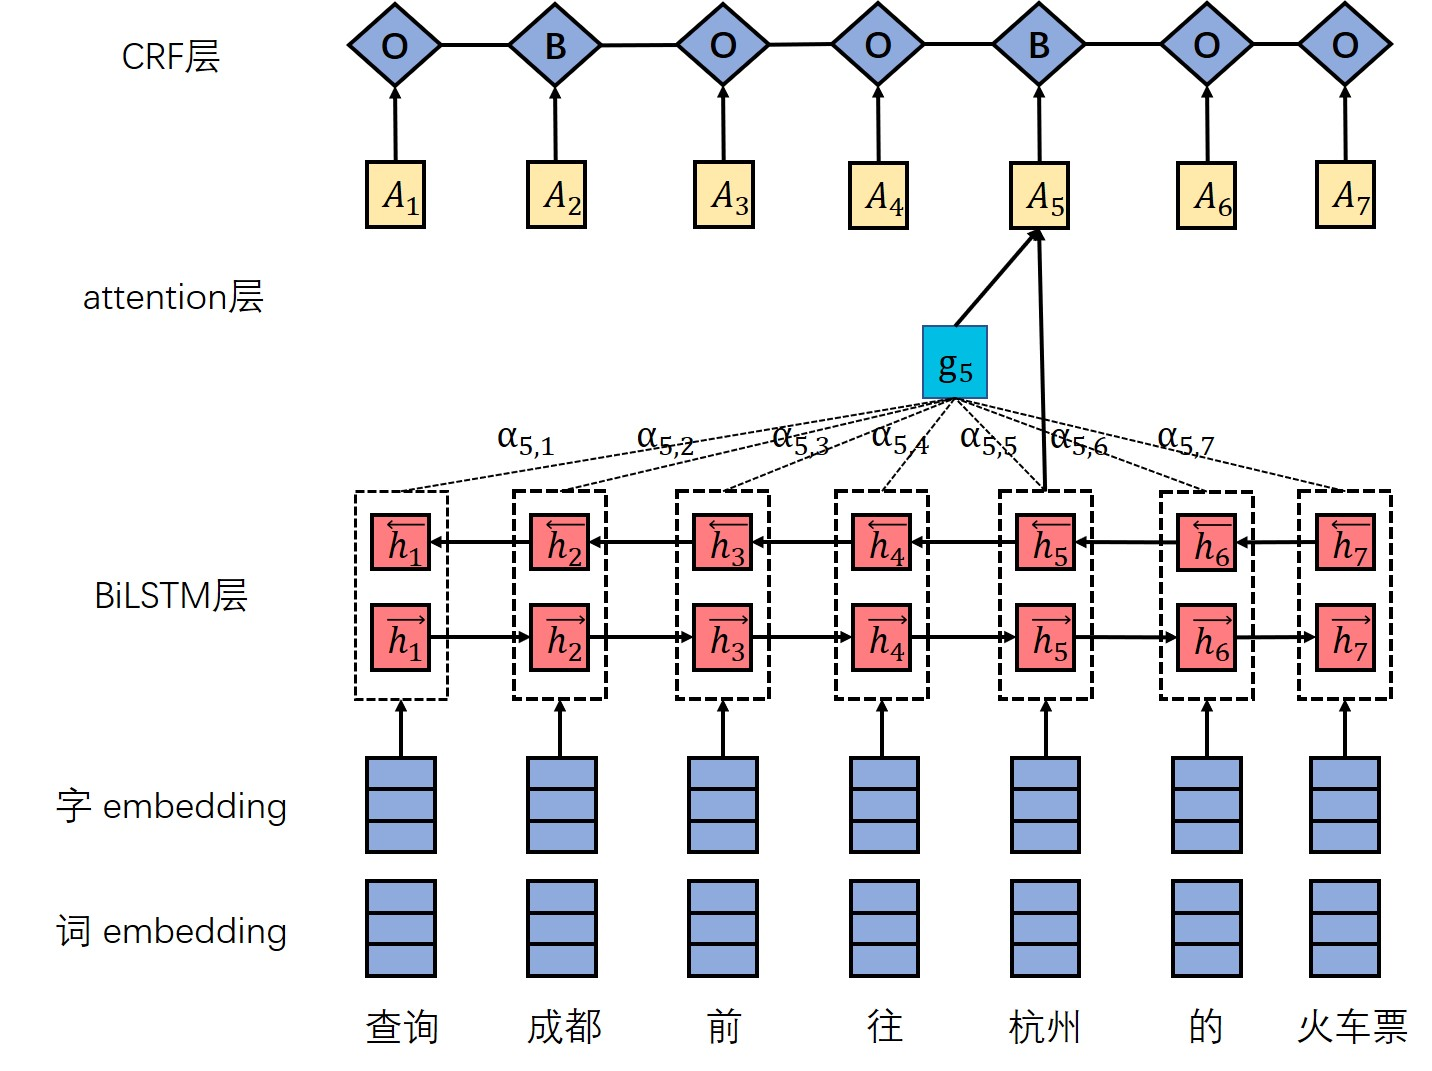
\includegraphics[scale=0.5]{./images/blstm-att-crf.jpg}
  \caption{参数填充模型}
  \label{fig:blstm-att-crf}
\end{figure}

1)输入层与embedding层

与前两个模型一致,首先,通过结巴分词工具得到词序列完成输入层的工作。本模型除了词嵌入处理外,引入了字向量。设
$\mathbf{e}_{i}^{w}$表示用户输入语句词序列中第i个词的向量,$\mathbf{e}_{i}^{c}$指用户输入语句词序列中第i个词中所有字向量的表示,
则embedding层第i个词向BiLSTM层输入可表示为:
\begin{equation}
  \mathbf{x}_{i}=[\mathbf{e}_{i}^{w} ;\mathbf{e}_{i}^{c}]
\end{equation}
其中,我们会单独用另一个双向LSTM(图中未标出),输入为一句话的字向量序列,对于单词$w_i$的字向量$c_t(i,1),\dots,c_t(i,len(i))$(len(i)为词语的长度),
可以得到$\overrightarrow{\mathbf{h}}_{t(i, 1)}^{c}$,\dots,$\overrightarrow{\mathbf{h}}_{t(i, len(i))}^{c}$
和$\overleftarrow{\mathbf{h}}_{t(i, 1)}^{c}$,\dots,$\overleftarrow{\mathbf{h}}_{t(i, len(i))}^{c}$ ,上式中的$\mathbf{e}_{i}^{c}$由以下公式得出:
\begin{equation}
  \mathbf{e}_{i}^{c}=[\overrightarrow{\mathbf{h}}_{t(i, len(i))}^{c} ; \overleftarrow{\mathbf{h}}_{t(i, 1)}^{c}]
\end{equation}

2)BiLSTM-attention层

嵌入层的向量输入到双向LSTM网络中后,对每一个词$\mathbf{e}_{i}^{w}$,前向LSTM输出带有从左往右语义的向量$\overrightarrow{\mathbf{h}}_{i}$,
后向LSTM输出带有从右往左语义的向量$\overleftarrow{\mathbf{h}}_{i}$,我们将这两个向量拼接得到$\mathbf{h}_{i}=[\overrightarrow{\mathbf{h}}_{i} ;\overleftarrow{\mathbf{h}}_{i}]$
并对$\mathbf{h}_{i}$做attention处理。
attention层主要运算工作是计算词与词之间的语义相似的,这里代表着一个词$\mathbf{e}_{i}^{w}$的向量便是$\mathbf{h}_{i}$,则词i与词j之间的attention权重$α_{i,j}$可由下式得到:
\begin{equation}
\alpha_{t, j}=\frac{\exp \left(\operatorname{score}\left(\mathbf{h}_{i}, \mathbf{h}_{j}\right)\right)}{\sum_{k} \exp \left(\operatorname{score}\left(\mathbf{h}_{i}, \mathbf{x}_{k}\right)\right)}
\end{equation}
\begin{equation}
  \operatorname{score}(\mathbf{h}_{i}, \mathbf{h}_{j}))=\tanh \left(\mathbf{W}_{a}\left[\mathbf{h}_{i} ; \mathbf{h}_{j}\right]\right)
\end{equation}
attention权重由带有参数$\mathbf{W}_{a}$的感知器计算得到,以此来表示在理解目前词i时应该放多少注意力在词j上:
\begin{equation}
  \mathbf{g}_{i}=\sum_{j=1}^{N} \alpha_{i, j} \mathbf{h}_{j}
\end{equation}
于是我们得到了拥有全局视野的词i的向量表示$\mathbf{g}_{i}$,将它与$\mathbf{h}_{i}$拼接得到向量$\mathbf{a}_{i}=[\mathbf{g}_{i} ;\mathbf{h}_{i}]$作为CRF层的输入。
(这里选用字母a的原因时做了attention处理)

3)CRF层

在模型的最后,添加了CRF层以对所有可能的标记路径中的最佳标记进行解码。
设$\mathbf{P}$是分数矩阵,矩阵的元素$P_{i,j}$是句子中第i个单词被标记为第j个标签的分数。 
同时引入一个标记转换矩阵$\mathbf{T}$,其中$T_{i,j}$表示上下连续两个单词中从上一个被标记i到下一个被标记j的转换分数,
而$T_{0,j}$表示从标记j作为开始的分数,该转换矩阵将做为模型的参数被训练。 
句子$\mathbf{X}$的被标记为$\mathbf{X}=(y_1,y_2,\dots,y_n)$的得分可由下式得出:
\begin{equation}
  s(\mathbf{X}, \mathbf{y})=\sum_{i=1}^{n}\left(T_{y_{i-1}, y_{i}}+P_{i, y_{i}}\right)
\end{equation}
之后可以通过softmax函数推导出$\mathbf{X}$的被标记为$\mathbf{X}=(y_1,y_2,\dots,y_n)$的概率:
\begin{equation}
  p(\mathbf{y} \mid \mathbf{X})=\frac{e^{s(\mathbf{X}, \mathbf{y})}}{\sum_{\tilde{\mathbf{y}}} e^{s(\mathbf{X}, \tilde{\mathbf{y}})}}
\end{equation}
在训练时,模型的目标是使正确标注信息的概率最大。









